\documentclass{standalone}

\usepackage{tikz}
\usepackage{circuitikz}

\tikzset{block/.style = {draw, fill=white, very thick, rectangle, minimum height=1cm, minimum width=2cm},
         lblock/.style={draw,fill=white,very thick, rectangle, minimum height=3cm, minimum width=1cm},
         sum/.style= {draw, fill=white, very thick, circle, node distance=0.5cm}}

         
\begin{document}
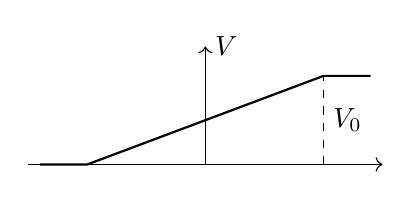
\begin{tikzpicture}[scale=1.5]
    \draw[->](-1.5,0)--(1.5,0);
    \draw[->](0,0)--(0,1)node[right]{$V$};
    \draw[thick](-1.4,0)--(-1,0)--(1,0.75)--(1.4,0.75);
    \draw[dashed](1,0)--(1,0.75)node[midway, right]{$V_0$};
\end{tikzpicture}
\end{document}